\documentclass{pnastwo}

% Including pdf figures
\usepackage{graphicx}

% Including math features
\usepackage{amsmath}
\usepackage{amssymb}
\usepackage{amsfonts}
\usepackage{graphicx}

% Including male & female symbols
\usepackage{wasysym}

%referencing SupMat
\usepackage{xr}
\externaldocument{SupMat}

% Including pdf figures
\usepackage{graphicx}
\usepackage{pdfpages}
% Math stuff
\usepackage{amsmath}
\usepackage{amssymb}
\usepackage{amsfonts}

% Bibliographies
%\usepackage[]{natbib}
%\bibpunct{[}{]}{,}{n}{}{;} 
%Fonts
%\usepackage[comma,sort&compress]{natbib}

\usepackage{lineno} %gives line numbers with \lineno command

\usepackage{setspace}
%\onehalfspace

\DeclareMathOperator{\Var}{Var}
\DeclareMathOperator{\Cov}{Cov}

\renewcommand{\bibitfont}{\fontsize{6pt}{9pt} \bibfont\slshape}



% Formats equations as (#)
% \renewcommand{\eqref}[1]{\textup{{\normalfont(\ref{#1}}\normalfont)}}

% Formats equations as bold #
\renewcommand{\eqref}[1]{\textup{\bf{\ref{#1}}}}

%%% font setup in order to make the article printable
%\usepackage{mathptmx}
%\usepackage{helvet}
%\renewcommand\bibfont{\fontsize{6pt}{9pt}\bfseries\sffamily}
%\renewcommand{\bibitfont}{\bibfont\slshape}
%\renewcommand{\bibbffont}{\bibfont}
%%%

\renewcommand{\bibitfont}{\fontsize{6pt}{9pt} \bibfont\slshape}

%------------------------------------------------
% DO NOT EDIT THIS SECTION
%------------------------------------------------

%% For PNAS Only:
\url{www.pnas.org/cgi/doi/10.1073/pnas.0709640104}
\copyrightyear{2008}
\issuedate{Issue Date}
\volume{Volume}
\issuenumber{Issue Number}

%----------------------------------------------------------------------------------------

\begin{document}

\title{The Role of Pollen and Sperm Competition in Sex Chromosome Evolution}
\author{
Michael F Scott\affil{1}{University of British Columbia, Vancouver BC, Canada}\affil{2}{corresponding author: mfscott@biodiversity.ubc.ca},
\and
Sarah P.~Otto\affil{1}{}}

%\maketitle

\significancetext{
%[120 word max] 
One feature that characterizes many sex chromosome systems is that, along most of the length, there is no recombination with the opposite sex chromosome.
The typical explanation for this phenomenon entails differences in selection between the sexes. 
However, selection during the haploid phase of males and females can also be strikingly divergent, with male-derived pollen/sperm experiencing particularly intense competition. 
We show that competition between pollen/sperm can favour extreme suppression of recombination between sex chromosomes. 
Extremely suppressed recombination allows strong associations between pollen/sperm beneficial alleles and the male-determining region (Y or Z), which results in biased sex ratios in XY systems. 
Thus, we provide predictions about the rate of sex chromosome evolution and genomic location of pollen/sperm expressed genes.
}


\maketitle

\begin{article}

\noindent
%$^1$ Department of Botany, University of British Columbia, \#3529 - 6270 University Boulevard, Vancouver, BC, Canada V6T 1Z4

\noindent
%$^2$ Department of Zoology, University of British Columbia, \#4200 - 6270 University Boulevard, Vancouver, BC, Canada V6T 1Z4

\noindent
%email: mfscott@biodiversity.ubc.ca. 

\noindent
%Contributions: MFS designed and analyzed the models and wrote the manuscript. 
%SPO assisted with model analysis and edited the manuscript.

%\newpage

%\linenumbers
%\modulolinenumbers[2]

\begin{abstract}
To date, research on the evolution of sex chromosomes has focused on sexually antagonistic selection, which has been shown to be a potent driver of the strata and reduced recombination that characterize many sex chromosomes
In this study, we expand our view of the forces driving sex chromosome evolution by considering also selection among haploids, which is likely to occur predominantly among male gametes in angiosperms and animals, i.e., during pollen or sperm competition.
We find that suppressed recombination is favoured on the sex chromosomes, even without selective differences between male and female diploids.
Reduced recombination is favoured because it creates a stronger association between haploid beneficial alleles and the male determining region (Y or Z), which experiences haploid selection most often. 
Similarly, reduced recombination creates linkage between alleles selected against in the haploid stage and the female determining region (X or W).
In XY systems, these associations also result in biased sex ratios at birth.
% ploidally antagonistic selection, in which an allele can be beneficial during the haploid phase and deleterious during the diploid phase. 
%Therefore, conflicts between haploid and diploid phases can be partially resolved by linking genes that are selected in both haploid and diploid phases with sex chromosomes. 
Overall, we predict that whether and how fast recombination suppression evolves on the sex chromosomes can depend on the degree of haploid competition, not just on selective differences between the diploid sexes.
Based on our models, sex chromosomes should become enriched for genes that experience haploid selection, as is expected for genes that experience sexually antagonistic selection.
Thus, we generate a number of promising predictions that can be evaluated in emerging sex chromosome systems. 
\end{abstract}


\keywords{recombination evolution|sex chromosomes|sperm competition|pollen competition|haploid selection|modifier model|evolutionary theory} % When adding keywords, separate each term with a straight line: |


%\newpage

\section*{Introduction}

In organisms with diploid genetic sex determination, recombination is typically suppressed between the X and Y chromosomes or Z and W chromosomes. 
Suppressed recombination appears to begin near the sex-determining region (SDR) and then expand to include larger segments of each sex chromosome \cite{Bergero:2007kr,Nam:2008ko,Lemaitre:2009ij,Wang:2012,Charlesworth:2013}. 
In the absence of recombination, the sex-limited chromosome (Y or W) accumulates deleterious mutations (including gene losses) within the non-recombining region and `genetic degeneration' occurs \cite{Rice:1996ke,Charlesworth:2000cc,Bachtrog:2006ed,Marais:2008hm}.
Thus, the selective forces driving reduced recombination on sex chromosomes are fundamental to our understanding of sex chromosome evolution. 

%In plants, recombination suppression is thought to occur during the establishment of the sex-determining region \cite{Charlesworth:2005cx,Charlesworth:2013,Charlesworth:2015dj}. 
%In particular, when separate sexes evolve from hermaphroditism, mutations to suppress both the male and female functions are required. 
%Reduced recombination between such loci is then favoured to avoid the production of offspring that are both male sterile and female sterile \cite{Nei:1969tb,Charlesworth:1978ut}.
%Here, we focus on the evolution of recombination between sex chromosomes after a sex-determining region has been established.  

Typically, selective differences between males and females have been evoked to explain the suppression of recombination around established sex-determining regions \cite{Fisher:1931jo,Bull:1983vi, Rice:1987hs}. 
Charlesworth and Charlesworth \cite{Charlesworth:1980} showed that loci where males and females differ in equilibrium allele frequency due to selection (for example, sexually antagonistic selection) should evolve complete linkage with the sex-determining locus via translocations or fusions. 
More recently, Lenormand \cite{Lenormand:2003ug} demonstrated that sex differences in allele frequencies at equilibrium are not required in order to favour reduced recombination with the sex-determining region.
%, rather that there must be a difference in selection on alleles when found in males and females. 
In fact, recombination suppression can evolve around the sex-determining region even if selection favours the same allele in both sexes as long as that allele is favoured more strongly in one sex than the other.  
In essence, these studies have demonstrated that suppressors of recombination can be favoured because they strengthen the association between the sex in which an allele is favoured and the chromosome that is present in that sex more often, e.g., between male beneficial alleles and the Y or Z and between female beneficial alleles and the X or W  \cite{Otto:2011ua}. 

While differences in selection between the diploid sexes has attracted the most theoretical and empirical attention, haploid gametes/gametophytes produced by males and females typically differ in the potential for selection because competition among pollen and sperm is particularly intense \cite{Mulcahy:1996ha,Bernasconi:2004dk,JOSEPH:2004haa}. 
To the extent that pollen and sperm success reflects differences in their haploid genotypes, selection among these gametes/gametophytes is qualitatively distinct from selection among diploid males. 
That is, diploids cannot be assigned fitness values that also account for the fitness of their haploid gametes \cite{Immler:2012tl}. 
In plants, selection among haploid male gametophytes is thought to be pervasive \cite{SKOGSMYR:2002ce,Moore:2011jt,Marshall:2016fe}; in \textit{Arabidopsis}, 60-70\% of all genes are expressed during the haploid phase \cite{Borg:2009jpa}, and pollen expressed genes exhibit stronger signatures of purifying selection and positive selection \cite{Arunkumar:2013iq,Gossmann:2014dua}.
For agricultural breeding, pollen has been exposed to a variety of selection pressures \textit{in vivo} and \textit{in vitro}, including temperature \cite{Hedhly:2004iv,Clarke:2004ir}, herbicides \cite{Frascaroli:2001ee}, metals \cite{Searcy:1985vt}, water stress \cite{Ravikumar:2003uo}, and pathogens \cite{Ravikumar:2012ej}, resulting in an increased frequency of resistant genotypes among the diploid sporophytic offspring. 
In animals, expression during the haploid sperm stage is traditionally thought to be suppressed \cite{Hecht:1998hz}, although recent evidence suggests that the extent and selective importance of postmeiotic gene expression may be underestimated \cite{Zheng:2001fi,JOSEPH:2004haa,Vibranovski:2010et,Immler:2014im}. 

The maintenance of polymorphism at loci that experience sex specific selection in both haploid and diploid phases was considered by Immler et al. \cite{Immler:2012tl}, demonstrating that polymorphisms can be maintained by sexually antagonistic selection or overdominance as well as by conflicting selection pressures in haploids and diploids (haploid-diploid conflict or ploidally antagonistic selection) or a combination of these selective regimes.  
In this study, we include selection during the male haploid phase (sperm or pollen competition) in models for the evolution of recombination with the sex-determining region (XY or ZW).

\section{Model Background}

Recombination evolution on sex chromosomes is usually modelled by considering a locus under selection, the sex-determining region, and another locus that modifies the recombination rate between them, where modifiers include inversions, fusions, hotspot changes, and changes to genes involved in double strand breaks and recombination repair.
%, which is typically assumed not to have any direct fitness effect. 
Thus, a general model includes three loci and the recombination rates between them, which is typically too complex to interpret without further simplifying assumptions \cite{Otto:2007tv}. 
Lenormand \cite{Lenormand:2003ug} assumed that the recombination rates between these loci are large relative to selection, such that the linkage disequilibrium between loci equilibrates on a faster timescale than changes in allele frequencies (a `quasi-linkage equilibrium' approximation). 
This analysis is most appropriate for selected loci that are far from the sex-determining region on sex chromosomes and when modifiers of recombination are weak and loosely linked (e.g., autosomal modifiers of recombination machinery). 
Secondly, Charlesworth and Charlesworth \cite{Charlesworth:1980} assumed that the selected locus is initially autosomal and then considered fusions with (or translocations to) the sex-determining region, where their analysis assumed these rearrangements became closely linked to the selected locus. 
Their model also corresponds to modifications on sex chromosomes (e.g., inversions) that change the recombination rate with the sex-determining region from a very high to a very low level. 
Finally, Otto \cite{Otto:2014jf} considered modifiers of recombination between the sex-determining region and selected loci when the linkage between them is initially very tight. 

Here, we study recombination evolution in a manner akin to Charlesworth and Charlesworth \cite{Charlesworth:1980} and Otto \cite{Otto:2014jf} except that we include a period of selection among haploid male gametes/gametophytes. 
The model of Lenormand \cite{Lenormand:2003ug} is very general and allows a period of haploid selection (assuming weak linkage); he recognizes but does not discuss the potential of such sex-specific haploid selection to favour suppressed recombination on sex chromosomes. 
Here, our goal is to complete the set of recombination evolution analyses that include a period of haploid pollen/sperm competition and explicitly describe why loci that experience haploid selection can drive the evolution of reduced recombination near sex-determining regions. 
Models where haploid selected loci and the sex-determining region can become tightly linked are particularly significant because sex in an XY sex determination system is determined by the chromosome carried by the successful pollen/sperm (after haploid selection). 
Thus, strong associations between haploid selected alleles and the sex-determining region (that can build up when linkage is tight) will cause diploid sex ratios to become biased, figure 1.  

\section*{Model}

%%%%%%%%%%%%%%%%%%%%%%%%%%%
% Consider replacing $w_{i}$ with $v_{i}$ throughout.
% Consider also $w_{i}^{m}$

We consider a modifier model in which the recombination rate between a locus under selection (selected locus, \textbf{A}, with alleles $A$ and $a$) and the sex-determining region (SDR) depends on the genotype at the modifier locus (\textbf{M}, with alleles $M$ and $m$). 
In our model, male haploid gametes/gametophytes experience selection according to their genotype at the \textbf{A} locus (see table \ref{tab:fitnesstable}) before random mating with female gametes/gametophytes. 
The resulting zygotes develop as males or females depending on their genotype at the sex-determining region. 
Diploid genetic sex determination systems are either male heterogametic (females XX and males XY) or female heterogametic (females ZW and males ZZ). 
There are therefore two asymmetries in the model, the sex in which haploid selection occurs and the sex which is heterogametic. 
%and our model also describes systems in which haploid selection occurs only among female gametes, with a corresponding change of male/female labelling. 
For simplicity, we primarily describe XY sex determination with male gametophytic selection (pollen/sperm competition), although we also present results for ZW sex determination and male gametophytic selection. 

After a period of selection among diploid males and females (table \ref{tab:fitnesstable}), meiosis with recombination occurs to produce haploid gamete/gametophytes. 
Because females are homozygous at the SDR (with XY sex determination), the only recombination event of consequence in females is between the \textbf{A} and \textbf{M} locus, which occurs at rate $R_{f}$. 
In males, recombination similarly occurs between the selected locus \textbf{A} and the modifier locus \textbf{M} at rate $R_{m}$. 
Recombination can also occur between the SDR and the \textbf{A} locus in males, this recombination rate is controlled by the modifier locus and is given by $r_{ij}$, where $ij$ is the genotype at the \textbf{M} locus ($MM$, $Mm$, or $mm$), allowing this recombination rate to evolve.  
Double recombination events in males occur at rate $\chi_{ij}$, such that any ordering of the loci or type of modifier (genic, inversion, fusion) can be modelled with appropriate choices of $\chi_{ij}$, $r_{ij}$, and $R_{m}$. 
We track the frequencies of $MA$, $Ma$, $mA$ and $ma$ genotypes among female eggs/ovules, male X-bearing sperm/pollen, and male Y-bearing sperm/pollen separately to allow sex-specific allele frequencies and disequilibria. 
The recursion equations describing the change in genotype frequencies after a single generation of this life cycle are provided in the Sup. Mat.

In our first analysis, we assume that selection is weak relative to the initial recombination rate ($r_{MM}$), such that allele frequency differences between males and females are small.
We then evaluate the spread of modifiers of recombination ($m$) that cause recombination rates to become very small (assuming $r_{Mm}$, $\chi_{Mm}$, and $R_{m}$ are all small). 
These modifiers could be translocations or fusions from autosomes to sex chromosomes or, if the selected locus (\textbf{A}) begins on the sex chromosome, inversions or expansions of the non-recombining region.
We assume that chromosomes are still able to disjoin regularly from their homologs during meiosis. 

In our second analysis, following Otto \cite{Otto:2014jf}, we assume that the \textbf{A} locus begins at equilibrium and in tight linkage with the SDR ($r_{MM}$ and $\chi$ are on the order of a small term, $\epsilon$). 
We then consider whether any modifiers can invade that increase this recombination rate slightly (where the change in recombination rate, $r_{Mm}-r_{MM}$, is on the order of $\epsilon$). 
The recombination rate between the modifier locus and these sex chromosome loci ($R_{f}$ and $R_{m}$) is not constrained. 
This analysis focuses on the final stages of sex chromosome evolution, asking when complete recombination is favoured or not. 
%Considering sexually antagonistic selection without haploid selection, \citet{Otto:2014jf} showed that there are some conditions (particularly overdominance in males) under which a small amount of recombination between the SDR and a selected locus can be favoured. 

\begin{figure}[t]     
 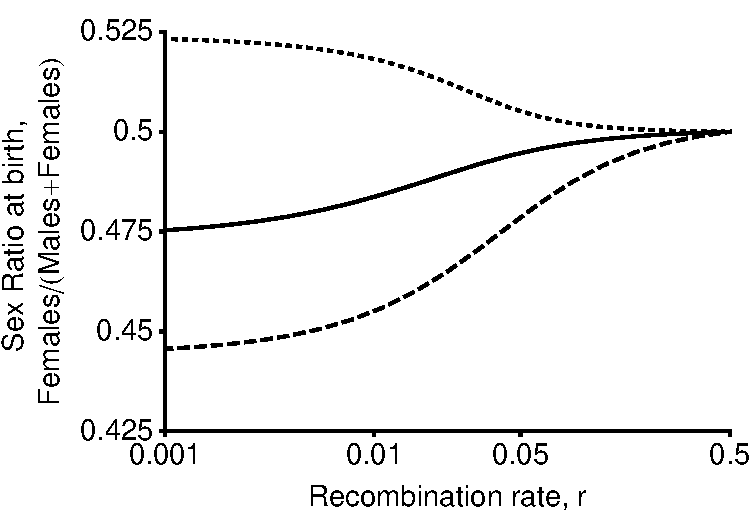
\includegraphics[width= 0.8 \linewidth]{Figures/sexRatioPlot.pdf} 
 \caption{
\textbf{The sex ratio at birth is biased by linkage between an XY sex-determining region (SDR) and a locus that experiences haploid selection during pollen/sperm competition (\textbf{A}).}
Here, we assume that the population is fixed for a particular modifier of recombination such that all individuals have the same recombination rate, $r$. We then allow the \textbf{A} locus to reach an equilibrium frequency and calculate the birth sex ratio.
Alleles with high fitness during pollen/sperm competition typically become associated with the Y, causing sex ratios to become male-biased (solid and dashed lines). 
However, female biased sex ratios can arise if the haploid-beneficial allele is also strongly female-beneficial, causing it to become associated with the X (dotted line). 
The parameters used in this plot are: 
solid line 
($w_{ij}^{m}=w_{ij}^{f}=w_{ij}$, $w_{aa}=1$, $w_{Aa}=0.97$, $w_{AA}=0.91$, $w_{a}=0.9$, $w_{A}=1$) 
dashed line 
($w_{ij}^{m}=w_{ij}^{f}=w_{ij}$, $w_{aa}=1$, $w_{Aa}=1.12$, $w_{AA}=1.24$, $w_{a}=0.8$, $w_{A}=1$), 
dotted line 
($w_{aa}^{m}=1$, $w_{Aa}^{m}=0.94$, $w_{AA}^{m}=0.8$, 
$w_{aa}^{f}=1$, $w_{Aa}^{f}=1.14$, $w_{AA}^{f}=1.2$ , $w_{a}=0.9$, $w_{A}=1$).
 }
 \label{fig:sexRatio} 
\end{figure}


\section*{Results}

%\subsection*{Fusions, Translocations and Other Large Effect Modifiers Bringing \textbf{A} into Tight Linkage with the SDR}

Considering a population originally fixed for the $M$ allele at the modifier locus, the frequency of the $A$ allele among X-bearing eggs/ovules, X-bearing sperm/pollen, and Y-bearing sperm/pollen is given by $p_{Xf}$, $p_{Xm}$, and $p_{Ym}$ respectively.
The spread of rare mutants that change the recombination rate can be evaluated using the leading eigenvalue, $\lambda$, of the system described by equations (A1c), (A1d), (A2c), (A2d), (A3c), and (A3d). 

Complete suppressors of recombination ($r_{Mm}=0$) that are closely linked to the \textbf{A} locus ($R_{f}=R_{m}=\chi=0$) experience the strongest selective force.  
These modifiers can bring either the $A$ or the $a$ allele into tight linkage with either the X or Y chromosome. 
Thus, the invasion of these mutants can be evaluated separately and is given by $\lambda_{ij}$, where $ij$ is the haplotype at the newly linked SDR and \textbf{A} loci. 

The spread of modifiers that create tight linkage between the Y and $A$ allele is given by

\begin{equation}
\lambda_{YA}=
\bar{w}_{YA}^{m}/\bar{w}^{m}
\label{eq:Yinv}
\end{equation}

\noindent
where $\bar{w}_{YA}^{m}$ is the marginal fitness of Y$A$ haplotypes and $\bar{w}^{m}$ is the mean fitness of males, see table \ref{tab:marginalFitnesses}.
Such modifiers will spread if $\lambda_{YA}>1$, which is true when $\bar{w}_{YA}^{m}>\bar{w}^{m}$.

Invasion of modifiers that create a strong linkage between the X and $a$ allele is determined by the largest solution to the characteristic polynomial \eqref{eq:Xcharpoly}.
For such modifiers, the leading eigenvalue $\lambda_{Xa}$ is greater than one if

\begin{equation}
\bar{w}_{Xa}^{mat,f}/\bar{w}^{f}+(\bar{w}_{Xa}^{mat,m}/\bar{w}^{m})(\bar{w}_{Xa}^{pat,f}/\bar{w}^{f}) >
2
\label{eq:XAinvconds}
\end{equation}

\noindent
where $\bar{w}^{f}$ is the mean fitness of females and $\bar{w}_{Xa}^{i,j}$ indicates the marginal fitness of X$a$ haplotypes when inherited from the mother ($i=mat$) or father ($i=pat$) and found in offspring of sex $j$
This condition demonstrates that the newly formed sex chromosome is able to invade if its marginal fitness is higher than average (once appropriately weighted across carriers of maternal and paternal copies). 
However, we have not yet considered constraints on the initial frequency of the $A$ allele. 

Next, we will consider the case where the \textbf{A} locus is initially at an intermediate frequency maintained by selection.
Polymorphisms can be maintained by a combination of sexually antagonistic selection, ploidally antagonistic selection, and/or overdominance \cite{Immler:2012tl}.
We then write $\lambda_{YA}$ in terms of the difference in fitness between haploid genotypes ($\delta_{H}=w_{A}-w_{a}$) and the difference in equilibrium allele frequency between Y-bearing pollen/sperm and ovules/eggs ($\delta=\hat{p}_{Ym}-\hat{p}_{Xf}$) where the caret indicates an equilibrium frequency. 
%In order to solve for the initial frequencies of the $A$ allele, we assume that linkage is initially loose between the SDR and \textbf{A} locus ($r_{MM}=1/2$, where the $M$ allele is initially fixed), such that segregation in males is random and $\hat{p}_{Xm}=\hat{p}_{Ym}=\hat{p}_{m}$ where the caret indicates an equilibrium frequency. 
We can then write equation \eqref{eq:Yinv}, for the invasion of modifiers that bring the $A$ allele into tight linkage with the Y chromosome, as

\begin{equation}
\lambda_{YA}=
1+\frac{r_{MM} w_{Aa}^{m}}{\hat{p}_{Ym} \bar{w}^{m}}\left(\delta +V_{m}\delta_{H}/\bar{w}_{H}  \right)
\label{eq:YinvEquil}
\end{equation}

\noindent
where $V_{m}=\hat{p}_{Ym} (1-\hat{p}_{Ym} )$ is the variance among Y-bearing pollen/sperm and $\bar{w}_{H}=(\hat{p}_{Ym} w_{A}+(1-\hat{p}_{Ym})w_{a})$ is the mean fitness of haploid male gametes/gametophytes.
If there is no selection among haploid genotypes ($w_{A}=w_{a}$), equation \eqref{eq:YinvEquil} is equivalent to equation (A3) in Charlesworth and Charlesworth \cite{Charlesworth:1980}, in which case these tightly linked Y$A$ haplotypes invade if the $A$ allele is more common in males than females ($\hat{p}_{m}-\hat{p}_{Xf}>0$), as expected if the $A$ allele is beneficial in males with sexually antagonistic selection. 
Here we also find an additional term, demonstrating that tight linkge is also favoured when the $A$ allele is beneficial during haploid selection ($w_{A}>w_{a}$), even in the absence of frequency differences between males and females ($\hat{p}_{Ym}=\hat{p}_{Xf}$), i.e., even when there is no difference in selection between diploid males and females. 

Here, in order to solve \eqref{eq:Xcharpoly} for $\lambda_{Xa}$, we will assume that linkage is initially loose between the SDR and \textbf{A} locus ($r_{MM}=1/2$), such that segregation in males is random and $\hat{p}_{Xm}=\hat{p}_{Ym}=\hat{p}_{m}$.
In the Sup. Mat we present equivalent results for cases where we do not assume that recombination is initially free ($r_{MM}<1/2$).
We will further assume that selection is weak, such that the difference in frequency between $A$ alleles in males and females ($\delta=\hat{p}_{m}-\hat{p}_{Xf}$) and the difference in fitness between haploid genotypes ($\delta_{H}=w_{A}-w_{a}$) are small ($\delta$ and $\delta_{H}$ of order $\epsilon^2$). 
Ignoring terms of order $\epsilon^3$ and higher

\begin{equation}
\lambda_{Xa} =
1+\frac{1}{3}\frac{w_{Aa}^{m}}{2 (1-\hat{p}_{m}) \bar{w}^{m}}\left( \delta +V_{m}\delta_{H} \right)
.
\label{eq:XinvEquil}
\end{equation}

\noindent
Thus, the same conditions that favour linkage between the Y and the $A$ allele, favour linkage between the X and the $a$ allele. Specifically, when the $a$ allele is more common in females ($\delta>0$, e.g., $a$ is a female beneficial allele) and when the $A$ allele is favoured during haploid competition ($\delta_{H}>0$). 
In the special case where there is no difference in selection between male and female diploids ($w_{ij}^m=w_{ij}^f=w_{ij}$), we can find an exact expression for $\lambda_{XA}$ by solving for $\hat{p}_{m}$ and $\hat{p}_{Xf}$ without assuming that selection is weak, which confirms the expectation from \eqref{eq:XinvEquil} that linkage between the X chromosome and alleles deleterious in haploid pollen/sperm is favoured by selection, see Sup. Mat. 

It may not be intuitively obvious why an association with the allele that is less fit during haploid selection should be favoured. 
This result comes from the fact that the $a$ allele is initially maintained at an equilibrium frequency when loosely linked to the SDR. 
At equilibrium, selection against $a$ in haploid male gametes/gametophytes must be balanced by selection in favour of $A$ in female and/or male diploids.
However, the X chromosome is found in males less often than an autosomal or loosely linked locus and therefore experiences haploid selection less frequently. 
Thus linkage between the $a$ locus and the X is favoured because it allows the $a$ allele to experience haploid selection less often. 
Similarly, equation \eqref{eq:YinvEquil} indicates that linkage between the Y, which experiences haploid selection most often, and a haploid beneficial allele is favoured. 

%Especially given the classic result of \textit{Hamilton, 1967} that, even if the $a$ allele is only favoured in male haploid gametes/gametophytes (n.b., \textit{Hamilton, 1967} considers male-specific drive, rather than haploid selection), it can spread on the X chromosome. 

As with previous analyses \cite{Charlesworth:1980,Charlesworth:1999kd,Lenormand:2003ug}, we find that the strength of selection in favour of recombination modifiers is strongest on Y chromosomes because these are always found in only one sex whereas the X will sometimes be found in males and sometimes in females. 
In particular, \eqref{eq:YinvEquil} and \eqref{eq:XinvEquil} differ by a factor of $1/3$ once we account for the difference between the probability of linkage arising with the $A$ allele, $p_{m}$, or the $a$ allele, $(1-p_{m})$. 
However, mutations causing linkage with the Y (e.g., fusions) should also arise at a lower rate because there are three times as many X chromosomes as Y chromosomes in the population, such that the overall establishment rate of recombination modifiers is the same on the X and Y \cite{Pennell:2015im}.


The tight linkage case considered above is the best case scenario for generating selection in favour of recombination suppressors. 
%Charlesworth and Charlesworth \cite{Charlesworth:1980} suggest that the tight linkage case considered above may be the best case scenario for generating selection in favour of recombination suppressors. 
For a few parameters, Charlesworth and Charlesworth \cite{Charlesworth:1980} find numerically that recombination suppressors spread, but at lower rates, if $R_{m}$ and $R_{f}$ are larger. 
Here, we find analytical results by assuming the recombination rates between the \textbf{A} locus, the \textbf{M} locus, and the SDR are small ($\chi$, $R_{m}$ and $R_{f}$ or order $\epsilon^3$). 
Neglecting terms of order $\epsilon^4$ and higher, the growth rate of such mutants ($\lambda\tilde{_{ij}}$) is.

\begin{subequations}
\begin{equation}
\begin{split}
\lambda\tilde{_{YA}} \approx&
\lambda_{YA}-
\frac{(1-\hat{p}_{m})w_{Aa}^{m}R_{m}}{\bar{w}^{m}}-\chi_{Mm}
\end{split}
\label{eq:Yinvr}
\end{equation}
\begin{equation}
\begin{split}
\lambda\tilde{_{Xa}} \approx
\lambda_{Xa}
%1+\frac{1}{3}
%\frac{w_{Aa}^{m}}{2 (1-\hat{p}_{m}) \bar{w}^{m}}\left( \delta +\hat{p}_{m} (1-\hat{p}_{m} )\delta_{H} \right) \\
%&
-\frac{\hat{p}_{m}}{3}\left(\frac{2w_{Aa}^{f}R_{f}}{\bar{w}^{f}} +\frac{w_{Aa}^{m}R_{m}}{\bar{w}^{m}} \right)-\frac{\chi_{Mm}}{3}
\end{split}
\label{eq:Xinv}
\end{equation}
\label{eq:XYinv}
\end{subequations}

\noindent
where $\lambda_{ij}$ corresponds to the tight linkage results \eqref{eq:YinvEquil} and \eqref{eq:XinvEquil}.
The additional terms in \eqref{eq:XYinv} illustrate that the spread of linked haplotypes is slowed when the alternative \textbf{A} allele recombines onto the modifier and SDR background (recombination rate $R_{m}$ or $R_{f}$) or when the modifier recombines onto the opposite sex chromosome (which occurs at rate $\chi_{Mm}$ in males). 
%This confirms the expectation from Charlesworth and Charlesworth \cite{Charlesworth:1980} that selection in favour of recombination suppression is strongest when linkage is tight. 
In figure \ref{fig:fusions}, we track the spread of a recombination modifier where $R_{m}, R_{f}, \chi, r_{Mm} \neq 0$, such that both  \textbf{M} alleles and both \textbf{A} alleles can recombine onto both sex chromosomes. As predicted from equation \eqref{eq:XYinv}, a recombination suppressor increases in frequency and the X and Y chromosomes become associated with the $a$ and $A$ alleles, respectively. 


\begin{figure}
 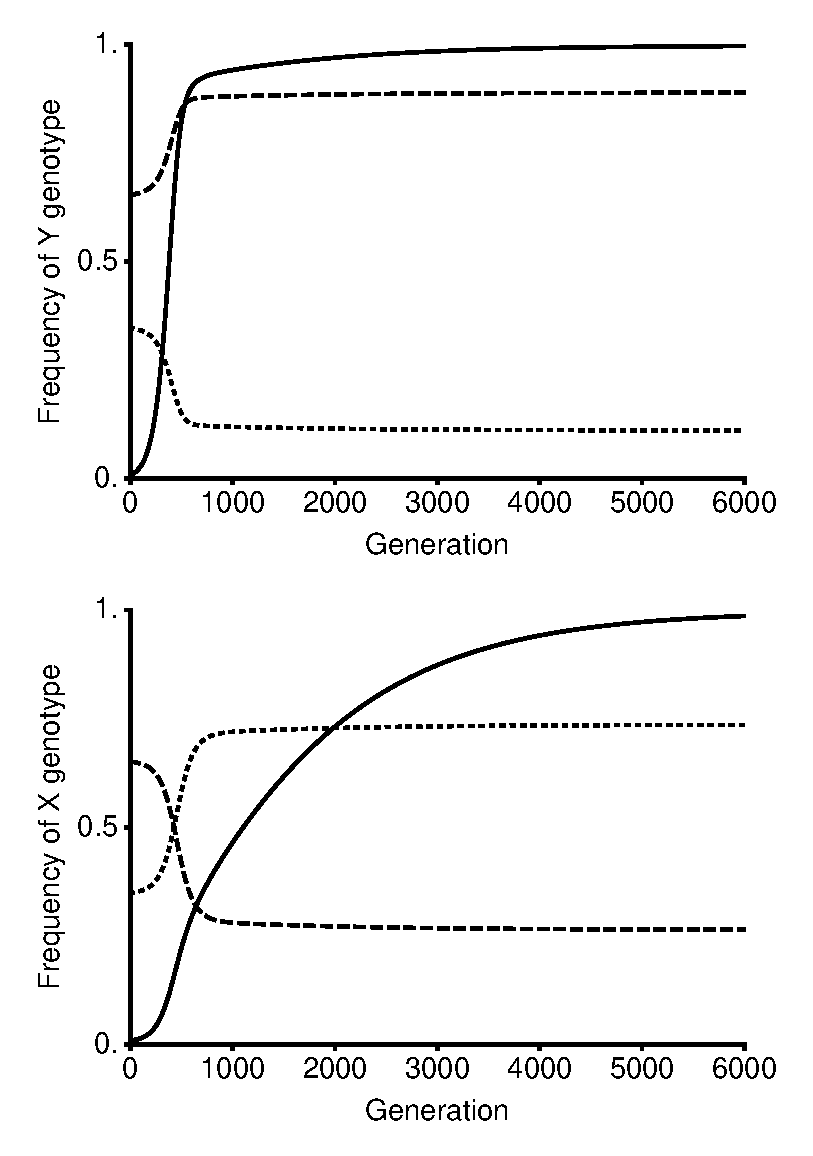
\includegraphics[width= 0.8 \linewidth]{Figures/fusion.pdf} 
 \caption{
 \textbf{A modifier that reduces the recombination rate between the \textbf{A} locus and the SDR can spread to fixation despite causing sex ratios to become biased.} Here, we iterate the recursion equations \ref{eq:recXf}, \ref{eq:recXm}, \ref{eq:recY} to track the change of genotype frequencies among X-bearing female haploids ($X_{i}^{f}$), X-bearing male haploids ($X_{i}^{m}$), and Y-bearing male haploids ($Y_{i}^{m}$), respectively. 
 Across this plot, X-bearing haploids in males and females have very similar haplotype frequencies so we plot $X_{i}^{m}$ only.
 We assume that the population initially has loose linkage between the \textbf{A} locus and the SDR ($r_{MM}=0.5$, where $M$ is initially fixed) and allow allele frequencies to reach a polymorphic equilibrium. 
 We then introduce a modifier allele $m$ that reduces the recombination rate between \textbf{A} locus and the SDR ($r_{Mm}=r_{mm}=0.01$); in generation 0, $m$ is at frequency $0.01$ and in linkage equilibrium with $M$.
 We assume that the \textbf{M} locus lies between the \textbf{A} locus and the SDR such that $\chi_{ij}=(r_{ij}-R_{m})/(1-2R_{m})$, where $R_{m}=R_{f}=0.005$.
Fitness parameters are as in the solid line in figure \ref{fig:sexRatio}. That is, there are no differences in selection between diploid sexes and selection is ploidally antagonistic with $A$ favoured by haploid selection, thus $\hat{p}_{Xf}=\hat{p}_{Xm}=\hat{p}_{Ym}$ initially, see Sup. Mat. 
Lines show the frequencies of the $A$ allele (dashed), the $a$ allele (dotted) the recombination suppression mutant, $m$ (solid).
Due to continuing recombination between the \textbf{A} locus, \textbf{M} locus, and the SDR, a particular haplotype does not fix on the Y chromosome, as is the case when $r_{ij} = 0$ (see Sup. Mat.). 
However, after recombination has evolved to a lower level, the haploid beneficial allele ($A$, dashed lines) becomes more common on the Y and less common on the X.
}
 \label{fig:fusions} 
\end{figure}


We derive equivalent results for ZW sex chromosome systems (where males are ZZ and females are ZW) with a period of haploid selection among male gametes/gametophytes.
We again consider invasion of a modifier that creates tight linkage between the \textbf{A} locus and the \textbf{M} locus ($r_{Mm}$, $\chi$, $R_{m}$ and $R_{f}$ of order $\epsilon^3$) in a population in which linkage is initially loose between the SDR and \textbf{A} locus ($r_{MM}=1/2$).
Here, we present $\lambda_{Wa}$ and $\lambda_{ZA}$ under the same assumptions as \eqref{eq:XYinv}, where the difference in frequency of the $A$ allele between males and females and the difference in fitness between haploid genotypes are small ($\delta=\hat{p}_{Zm}-\hat{p}_{Wf}$ where $\delta$ and $\delta_{H}$ are of order $\epsilon^2$), yielding

\begin{subequations}
\begin{equation}
\begin{split}
\lambda\tilde{_{Wa}} \approx&
1+\frac{r_{MM}w_{Aa}^{f}}{(1-\hat{p}_{f}) \bar{w}^{f}}\left(\delta+V_{f}\delta_{H} \right)%\\
%&
-
\frac{\hat{p}_{f}w_{Aa}^{f}R_{f}}{\bar{w}^{f}}-\chi_{Mm}
\end{split}
\end{equation}
\begin{equation}
\begin{split}
\lambda\tilde{_{ZA}} \approx&
1+\frac{1}{3}
\frac{w_{Aa}^{f}}{2 \hat{p}_{f} \bar{w}^{f}}\left( \delta +V_{f}\delta_{H} \right) \\
&-\frac{(1-\hat{p}_{f})}{3}\left(\frac{2w_{Aa}^{m}R_{m}}{\bar{w}^{m}} +\frac{w_{Aa}^{f}R_{f}}{\bar{w}^{f}} \right)-\frac{\chi_{Mm}}{3}
\end{split}
\end{equation}
\label{eq:ZWinvEquil}
\end{subequations}

\noindent
where we discard terms of $O(\epsilon^4)$. 
$\lambda_{ZA}$ and $\lambda_{Wa}$ show that, when the $A$ allele is more common in males ($\delta>0$), linkage between the male Z chromosome and the $A$ allele and linkage between the female specific W chromosome and the $a$ allele are both favoured. 
In addition, linkage is favoured between the Z and the allele favoured during haploid selection ($A$ if $\delta_{H}>0$) and between the female specific W chromosome and the allele with low haploid fitness ($a$ if $\delta_{H}>0$). 

%After this modifier is established, the \textbf{A} locus is effectively sex-linked and the Y haplotype becomes fixed for the $a$ allele ($p_{Ym}=0$ is stable), as explored in the next section along with the X-bearing haplotypes. 

Finally, we evaluate the evolution of recombination during the final stages of sex chromosome evolution by considering the evolution of small amounts of recombination around the sex-determining region. 
Considering diploid selection alone, Otto \cite{Otto:2014jf} demonstrated that a small amount of recombination can be maintained by selection. 
Due to the asymmetrical inheritance pattern of sex chromosomes, an allele that is fixed on a Y chromosome (e.g., the $A$ allele) can also be favoured on the X during selection in females, even if the X is fixed for the alternative allele (e.g., the $a$ allele). 
With diploid selection only, this requires that the X-specific allele ($a$) is favoured during selection on the X in males, which only occurs when selection in males is overdominant.
Assuming, for example, that the Y is originally fixed for the $A$ allele, recombination with the sex-determining region produces X$A$ and Y$a$ haplotypes in pollen or sperm. 
Although Y$a$ haplotypes always have low fitness, X$A$ haplotypes can experience a short term advantage because they next experience selection in females and selection in females can favour the $A$ allele.
For a subset of parameters, the cost of producing low fitness sons can be outweighed by this transient fitness advantage in daughters, allowing modifiers of recombination that increase recombination to invade if sufficiently loosely linked to the sex-determining region, for further discussion see \cite{Otto:2014jf}.
Here, we perform a similar analysis in which there is also a period of selection among male haploids.

We find that mutants that increase the recombination rate are not typically favoured by selection. 
In particular, when the modifier locus is tightly linked to the \textbf{A} locus ($R_{f} \approx 0$), only mutants that suppress recombination can spread.
In addition, if the allele that is fixed on the Y (e.g., $A$) is favoured by selection on the X in males ($w_{AA}^{m}>w_{Aa}^{m}$) but not during selection among haploids ($w_{a}>w_{A}$) increased recombination is never favoured. 
However, if these conditions are not met there are some parameters under which increased recombination is favoured by selection (figure \ref{fig:combined}). 

Assuming that the $A$ allele is initially fixed on the Y, increased recombination is favoured when the cost of producing Y$a$ pollen/sperm is be outweighed by selection in favour of X$A$ pollen/sperm.
%One might not expect selection to favour X$A$ haplotypes because an $A$ allele on an average X background should either have the same fitness as an $a$ allele (when a polymorphism is maintained on the X) or lower fitness (when $A$ is fixed on the X). 
%However, an X$A$ haplotype created by recombination in males is found in a male haploid (pollen or sperm), not on an average X background (which is weighted across X-bearing male sperm/pollen and female eggs/ovules). 
If $R_{f}$ and $R_{m}$ are small, the modifier remains linked to the haplotypes it creates (X$A$ and Y$a$), which always leads to a net long term disadvantage. 
When $R_{f}$ and $R_{m}$ are sufficiently large (e.g., autosomal modifiers), a modifier that increases recombination can gain a short term benefit from being found on X$A$ pollen/sperm before recombining onto a different background. 
X$A$ pollen or sperm can have a short term advantage if they have high fitness during haploid competition and/or high fitness in female diploids (all X-bearing pollen/sperm will form female diploids). 
Increased recombination is only consistent with X$A$ being favoured during haploid selection and/or selection in females, see Sup. Mat. 
For most parameters with or without haploid selection, X$A$ pollen/sperm either have no fitness advantage or have a transient fitness advantage that is outweighed by the cost of producing low-fitness Y$a$ pollen/sperm. 
Thus, increased recombination does not usually evolve. 
However, with selection among haploids, it is possible for a small amount of recombination to be favoured under a less restrictive set of selective regimes in diploids, including overdominance, sexually antagonistic selection and ploidally antagonistic selection. 

\section*{Discussion}

Even in predominantly diploid organisms such as animals and angiosperms, there is considerable potential for selection among haploid male gametes (sperm/pollen). 
Here, we demonstrate that linkage between the diploid sex-determining region (XY or ZW) and a locus that experiences haploid selection is typically favoured by selection. 
Thus, along with selective differences between diploid sexes, selection among haploids could be a potent driver of recombination suppression on sex chromosomes.

%Following \citet{Charlesworth:1980}, we considered extreme recombination modifiers that bring an initially loosely linked polymorphic locus into tight linkage with the sex-determining region. 
%We find that alleles favoured during haploid selection should become linked to the male sex chromosome (Y or Z), which experiences haploid selection most often, and that alleles disfavoured during haploid selection should become linked to the Z or W chromosome, which experiences haploid selection least often. 
%Indeed, the analysis of \citet{Lenormand:2003ug}, which assumes recombination rates are large relative to selection and modified by a small amount, also shows that reduced recombination is favoured when haploid selection occurs in one sex, even for loci not maintained at a polymorphic equilibrium by selection, (e.g., during the spread of beneficial mutations). 

In ZW sex determination systems, the sex ratio among diploids is unaffected by selection among male haploids. 
However, in XY sex determination systems, the number of males and females in each generation depends on the frequency of X and Y gametes after haploid selection. 
Despite this, we find that selection on recombination modifiers is not primarily driven by balancing the sex ratio of diploids.
In fact, the evolution of recombination suppression should lead to Y-bearing gametes/gametophytes that have high fitness during haploid selection.
Thus, we predict that sex ratios at birth can become male biased in the early stages of sex chromosome evolution. 

Biased flowering sex ratios, especially male-biased sex ratios, are common among dioecious plants \cite{Field:2013cc}.
However, in \textit{Rumex}, more intense pollen competition appears to result in more female biased sex-ratios among the progeny \cite{Conn:1981uw,Stehlik:2006to,Field:2012fd}. 
This phenomenon may reflect the accumulation of deleterious mutations on the Y-chromosome following recombination suppression \cite{Lloyd:1974tz,Stehlik:2005ul}, as suggested by the prevalence of female sex ratio bias in species with heteromorphic rather than homomorphic sex chromosomes \cite{Field:2013cc}. 
Thus, the net effect of experimentally manipulating the intensity of haploid selection may depend on the stage of sex chromosome degeneration, as well as the alleles associated with the Y. 
The increasing availability of sex-linked markers should allow sexes to be identified before reproductive maturity in plants, thus allowing changes in the sex ratio to be directly evaluated across haploid and diploid phases in species with differing degrees of Y chromosome degeneration.

The emergence of both haploid expression profiles \cite{JOSEPH:2004haa,Borg:2009jpa} and a larger number of sex chromosome systems \cite{Ming:2011iy,Charlesworth:2013,Charlesworth:2015dj,Bachtrog:2014bx,Vicoso:2015hf} provides an excellent opportunity to evaluate whether sex chromosomes are enriched for genes selected during the haploid phase, as predicted by our models. 
If possible, a stronger signal of association with sex-determining regions should occur among loci explicitly shown to exhibit variation in haploid competitive ability \cite{Travers:2001vx} or loci where mutants affect fitness in both haploid and diploid phases \cite{Muralla:2011ks}. 
Finally, we predict that the strength of haploid competition partly determines whether and how fast recombination suppression evolves.
Evaluating a related hypothesis, Lenormand and Duthiel \cite{Lenormand:2005vb} correlate heterochiasmy (differences in autosomal recombination between sexes) with the degree of sex specific haploid selection, using outcrossing rate as a proxy for male haploid selection. 
We would predict a similar pattern for recombination suppression around sex-determining regions. 
Estimates of pollen limitation could also be used as proxy for the intensity of haploid competition \cite{Vamosi:2006hi,Friedman:2009eg}. 

As in a previous analysis by Otto \cite{Otto:2014jf}, we find that a small amount of recombination can be selectively maintained around the sex-determining region. 
Otto \cite{Otto:2014jf} considered only diploid selection and found that overdominance in males was required for recombination to be selectively maintained. 
Here, we include a period of selection among haploids and find that increased recombination can be favoured with various forms of selection among diploids, including sexually antagonistic selection and ploidally antagonistic selection (figure \ref{fig:combined}), as long as the allele fixed on the Y is favoured in haploids and/or females. 
However, increased recombination is never favoured when modifiers of recombination act locally, such that they are also closely linked to the sex-determining region. 
Therefore, while these dynamics may influence the maintenance of small amounts of recombination around sex-determining regions when polymorphisms with the right form of selection arise (e.g., within the coloured regions in figure \ref{fig:combined}), suppressed recombination will be favoured in most circumstances. 


%In our models, and in most models for the evolution of recombination, modifiers of recombination are assumed not to have direct effects on fitness. 
%However, fusions and other chromosomal rearrangements can alter the number and position (acrocentric or metacentric) of active centromeres, which can lead to biased segregation during meiosis \cite{Wyttenbach:1998uj,PardoManueldeVillena:2001gn,PardoManueldeVillena:2001ti,Yoshida:2012cz}. 
%This meiotic drive either creates direct selection for or against these extreme recombination modifiers, which could overwhelm the selective consequences of recombination modification. 
%This is one reason why the rate of fusions with sex chromosomes may not primarily reflect the benefits of reduced recombination \cite{Pennell:2015im}.

%Mention: UV sex chromosomes

%In addition to loci with polymorphisms maintained by sexually antagonistic selection, loci with polymorphisms maintained by heterozygote advantage have been shown to evolve linkage with the sex-determining region if there is inbreeding \cite{Charlesworth:1999kd}. 
%Because the heterogametic sex is heterozygous at the sex-determining region (XY or ZW), linkage with this region preserves heterozygosity in the face of inbreeding. 

%Also Grossen study, "recombination in sex reversed individuals evolves towards zero in the presence of sexually antagonistic selection but towards a positive value when deleterious mutations were present as well. Given that the fitness effects of deleterious mutations were multiplicative and equal in the two sexes, deterministic models would predict no change in recombination, leading Grossen et al. (2012) to conclude that stochastic effects were responsible for the maintenance of recombination in their simulations (i.e. Muller's Ratchet and related Hill-Robertson effects)."

%In addition to the evolution of recombination suppression on sex chromosomes, sexually antagonistic selection has been implicated in the transition of genetic sex-determining systems between chromosomes. 
%In particular, a new male determining locus can spread if it arises in linkage with a locus experiencing sexually antagonistic selection \cite{vanDoorn:2007eu}. 
%Our results suggest a promising mechanism for future investigation, in which new male determination loci can arise close to loci experiencing haploid selection. 

Meiotic drive is not exactly equivalent to a period of haploid selection. In particular, meiotic drive can only occur in heterozygotes and often involves an interaction with a separate susceptible/resistant locus \cite{Bull:1983vi}.
However, meiotic drive is also usually sex specific, either acting during spermatogenesis in males or polar body formation in females. 
In this respect, we expect loci experiencing meiotic drive to behave similarly to those experiencing haploid selection. 
In particular, we predict that selection should favour linkage between alleles favoured by drive and the sex chromosome for the sex in which drive occurs (e.g., with the Y or Z when drive occurs during spermatogenesis). 
Despite theoretical interest in related topics \cite{Feldman:1989gm,Haig:2010em,Brandvain:2012hh,Patten:2014tn,Rydzewski:2016csa}, such as the evolution of recombination between an X chromosome that experiences drive and another selected locus \cite{Feldman:1989gm,Rydzewski:2016csa}, this process has yet to be explicitly modelled and is worthy of future exploration. 
%Although it should be noted that meiotic drivers may be more common on sex chromosomes for other reasons \cite{Hurst:1991uh}, for example, because meiotic drive often occurs via interactions with a susceptible allele on the homologous chromosome, divergence between sex chromosomes may provide a particularly large source of suitable targets for drive \cite{Burt:2006}. 
%Finally, Ubeda et al. \cite{Ubeda:2015fx} demonstrate that new male determining alleles can be favoured when linked to a locus that experiences drive in males, transitioning between environmental and genetic sex determination systems. Again, we would also expect new genetic sex determination loci to be favoured in systems with environmental sex determination if they arise near loci that experience selection in male gametophytes. 
%Overall, these results suggest that we can expand our view of sex chromosome evolution to incorporate sex specific haploid selection and meiotic drive as well as sex specific selection in diploids. 

Overall, as well as providing several predictions, our model offers a new perspective on drivers of sex chromosome evolution. 
Traditionally, sex differences in selection are thought to provide the raw material driving recombination suppression on sex chromosomes.
%A traditional view would conclude that the strength of sex differences in selection can determine how fast recombination suppression evolves on sex chromosomes. 
However, even where diploid sexes exhibit very few morphological or ecological differences, the selective environment of their haploid gametes may be very divergent.
We have shown that this condition - differences in fitness among pollen or sperm - should also favour suppressed recombination. 
Consequently, our view of sex chromosome evolution is expanded to incorporate the degree of sex specific selection in haploids along with that in diploids.  


%Note on ploidally-antagonistic selection, drop? (agricultural breeding moved to intro.)
%We find that recombination suppression can evolve even when there is no difference in selection between diploid sexes, in which case polymorphisms can be maintained by overdominance or ploidally-antagonistic selection (Appendix 1).
%Intralocus haploid-diploid conflict requires that genes under selection in the haploid phase are also selected in the diploid phase. 
%Of the genes expressed during male gametophyte (pollen) development, approximately 90\% are also expressed in the diploid sporophytic stage \cite{Borg:2009jpa}.
%For agricultural breeding, pollen has been exposed to a variety of selection pressures in vivo and in vitro, including temperature \cite{Hedhly:2004iv,Clarke:2004ir}, herbicides \cite{Frascaroli:2001ee}, metals \cite{Searcy:1985vt}, water stress \cite{Ravikumar:2003uo}, and pathogens \cite{Ravikumar:2012ej}, resulting in an increased frequency of resistant genotypes among the diploid sporophytic offspring, such that systematic changes in these environments between haploid and diploid stages could lead to antagonistic selection. 
%In a common environment, \citet{Travers:2001vx} show that an allele at the phophoglucoisomerase locus in \textit{Clarkia unguiculata} is favoured during pollen competition but causes reduced seed production by diploid sporophytes. 
%While selection may most often act in the same direction in both phases, we focus on loci that experience antagonism because alleles can be maintained at high frequencies and thus account for substantial genetic variation that is sustained for long time periods. 

\subsection*{Acknowledgements}

Funding for this project was provided by the University of British Columbia and by a Natural Sciences and Engineering Research Council of Canada grant to SPO.

%\bibliographystyle{pnas}
%\bibliography{Sex_Chromosomes.bib}

\begin{thebibliography}{20}

\bibitem{Bergero:2007kr}
Bergero R, Forrest A, Kamau E, Charlesworth D
 (2007) {Evolutionary strata on the X chromosomes of the dioecious
  plant \textit{Silene latifolia}: evidence from new sex-linked genes}.
 \textit{Genetics} 175:1945--1954.

\bibitem{Nam:2008ko}
Nam K, Ellegren H
 (2008) {The chicken (\textit{Gallus gallus}) Z chromosome contains at
  least three nonlinear evolutionary strata}.
 \textit{Genetics} 180:1131--1136.

\bibitem{Lemaitre:2009ij}
Lemaitre C, {et~al.}
 (2009) {Footprints of inversions at present and past pseudoautosomal
  boundaries in human sex chromosomes}.
 \textit{Genome Biology and Evolution} 1:56--66.

\bibitem{Wang:2012}
Wang J, {et~al.}
 (2012) {Sequencing papaya X and Yh chromosomes reveals molecular
  basis of incipient sex chromosome evolution.}
 \textit{Proceedings of the National Academy of Sciences}
  109:13710--13715.

\bibitem{Charlesworth:2013}
Charlesworth D
 (2013) {Plant sex chromosome evolution.}
 \textit{Journal of Experimental Botany} 64:405--420.

\bibitem{Rice:1996ke}
Rice WR
 (1996) {Evolution of the Y Sex Chromosome in Animals}.
 \textit{BioScience} 46:331--343.

\bibitem{Charlesworth:2000cc}
Charlesworth B, Charlesworth D
 (2000) {The degeneration of Y chromosomes.}
 \textit{Philosophical transactions of the Royal Society of London.
  Series B, Biological sciences} 355:1563--1572.

\bibitem{Bachtrog:2006ed}
Bachtrog D
 (2006) {A dynamic view of sex chromosome evolution.}
 \textit{Current opinion in genetics {\&} development} 16:578--585.

\bibitem{Marais:2008hm}
Marais GAB, {et~al.}
 (2008) {Evidence for degeneration of the Y chromosome in the
  dioecious plant \textit{Silene latifolia}}.
 \textit{Current Biology} 18:545--549.

\bibitem{Fisher:1931jo}
Fisher R
 (1931) {The evolution of dominance}.
 \textit{Biological Reviews} 6:363.

\bibitem{Bull:1983vi}
Bull JJ
 (1983) \textit{{Evolution of sex determining mechanisms.}}
 (The Benjamin Cummings Publishing Company).

\bibitem{Rice:1987hs}
Rice WR
 (1987) {The accumulation of sexually antagonistic genes as a
  selective agent promoting the evolution of reduced recombination between
  primitive sex chromosomes}.
 \textit{Evolution} 41:911.

\bibitem{Charlesworth:1980}
Charlesworth D, Charlesworth B
 (1980) {Sex differences in fitness and selection for centric fusions
  between sex-chromosomes and autosomes}.
 \textit{Genetical Research} 35:205--214.

\bibitem{Lenormand:2003ug}
Lenormand T
 (2003) {The evolution of sex dimorphism in recombination.}
 \textit{Genetics} 163:811--822.

\bibitem{Otto:2011ua}
Otto SP, Pannell JR, Peichel CL, Ashman TL
 (2011) {About PAR: the distinct evolutionary dynamics of the
  pseudoautosomal region}.
 \textit{Trends in Genetics} 27:358--367.

\bibitem{Mulcahy:1996ha}
Mulcahy DL, Sari-Gorla M, Mulcahy GB
 (1996) {Pollen selection - past, present and future}.
 \textit{Sexual Plant Reproduction} 9:353--356.

\bibitem{Bernasconi:2004dk}
Bernasconi G
 (2004) {Evolutionary ecology of the prezygotic stage}.
 \textit{Science} 303:971--975.

\bibitem{JOSEPH:2004haa}
Joseph S, Kirkpatrick M
 (2004) {Haploid selection in animals}.
 \textit{Trends in Ecology {\&} Evolution} 19:592--597.

\bibitem{Immler:2012tl}
Immler S, Arnqvist G, Otto SP
 (2012) {Ploidally antagonistic selection maintains stable genetic
  polymorphism}.
 \textit{Evolution} 66:55--65.

\bibitem{SKOGSMYR:2002ce}
Skogsmyr I, Lankinen A
 (2002) {Sexual selection: an evolutionary force in plants?}
 \textit{Biological Reviews} 77:537--562.

\bibitem{Moore:2011jt}
Moore JC, Pannell JR
 (2011) {Sexual selection in plants}.
 \textit{Current Biology} 21:R176--R182.

\bibitem{Marshall:2016fe}
Marshall DL, Evans AS
 (2016) {Can selection on a male mating character result in
  evolutionary change? A selection experiment on California wild radish,
  \textit{Raphanus sativus}}.
 \textit{American journal of botany} 103:553--567.

\bibitem{Borg:2009jpa}
Borg M, Brownfield L, Twell D
 (2009) {Male gametophyte development: a molecular perspective}.
 \textit{Journal of Experimental Botany} 60:1465--1478.

\bibitem{Arunkumar:2013iq}
Arunkumar R, Josephs EB, Williamson RJ, Wright SI
 (2013) {Pollen-specific, but not sperm-specific, genes show stronger
  purifying selection and higher rates of positive selection than sporophytic
  genes in \textit{Capsella grandiflora}}.
 \textit{Molecular biology and evolution} 30:2475--2486.

\bibitem{Gossmann:2014dua}
Gossmann TI, Schmid MW, Grossniklaus U, Schmid KJ
 (2014) {Selection-driven evolution of sex-biased genes Is consistent
  with sexual selection in \textit{Arabidopsis thaliana}}.
 \textit{Molecular biology and evolution} 31:574--583.

\bibitem{Hedhly:2004iv}
Hedhly A, Hormaza JI, Herrero M
 (2004) {Effect of temperature on pollen tube kinetics and dynamics in
  sweet cherry, \textit{Prunus avium} (Rosaceae).}
 \textit{American journal of botany} 91:558--564.

\bibitem{Clarke:2004ir}
Clarke HJ, Khan TN, Siddique KHM
 (2004) {Pollen selection for chilling tolerance at hybridisation
  leads to improved chickpea cultivars}.
 \textit{Euphytica} 139:65--74.

\bibitem{Frascaroli:2001ee}
Frascaroli E, Songstad DD
 (2001) {Pollen genotype selection for a simply inherited qualitative
  factor determining resistance to chlorsulfuron in maize}.
 \textit{Theoretical and Applied Genetics} 102:342--346.

\bibitem{Searcy:1985vt}
Searcy KB, Mulcahy DL
 (1985) {Pollen selection and the gametophytic expression of metal
  tolerance in \textit{Silene dioica} (Caryophyllaceae) and \textit{Mimulus
  guttatus} (Scrophulariaceae)}.
 \textit{American journal of botany} 72:1700--1706.

\bibitem{Ravikumar:2003uo}
Ravikumar RL, Patil BS, Salimath PM
 (2003) {Drought tolerance in sorghum by pollen selection using
  osmotic stress}.
 \textit{Euphytica} 133:371--376.

\bibitem{Ravikumar:2012ej}
Ravikumar RL, Chaitra GN, Choukimath AM, Soregaon CD
 (2012) {Gametophytic selection for wilt resistance and its impact on
  the segregation of wilt resistance alleles in chickpea (\textit{Cicer
  arietinum} L.)}.
 \textit{Euphytica} 189:173--181.

\bibitem{Hecht:1998hz}
Hecht NB
 (1998) {Molecular mechanisms of male germ cell differentiation}.
 \textit{Bioessays} 20:555--561.

\bibitem{Zheng:2001fi}
Zheng Y, Deng X, Martin-DeLeon PA
 (2001) {Lack of sharing of Spam1 (Ph-20) among mouse spermatids and
  transmission ratio distortion}.
 \textit{Biology of Reproduction} 64:1730--1738.

\bibitem{Vibranovski:2010et}
Vibranovski MD, Chalopin DS, Lopes HF, Long M, Karr TL
 (2010) {Direct evidence for postmeiotic transcription during
  \textit{Drosophila melanogaster} spermatogenesis}.
 \textit{Genetics} 186:431--433.

\bibitem{Immler:2014im}
Immler S, Hotzy C, Alavioon G, Petersson E, Arnqvist G
 (2014) {Sperm variation within a single ejaculate affects offspring
  development in Atlantic salmon}.
 \textit{Biology letters} 10:20131040.

\bibitem{Otto:2007tv}
Otto SP, Day T
 (2007) \textit{{A biologist's guide to mathematical modeling in ecology
  and evolution}}
 (Princeton University Pres, Princeton, NJ).

\bibitem{Otto:2014jf}
Otto SP
 (2014) {Selective maintenance of recombination between the sex
  chromosomes.}
 \textit{Journal of Evolutionary Biology} 27:1431--1442.
 
 \bibitem{Charlesworth:1999kd}
B~Charlesworth and J~D Wall. (1999)
{Inbreeding, heterozygote advantage and the evolution of neo-X and
  neo-Y sex chromosomes}.
\textit{Proceedings of the Royal Society B: Biological Sciences},
  266(1414):51--56.
 
 \bibitem{Pennell:2015im}
Matthew~W Pennell, Mark Kirkpatrick, Sarah~P Otto, Jana~C Vamosi, Catherine~L
  Peichel, Nicole Valenzuela, and Jun Kitano.
(2014) {Y fuse? Sex chromosome fusions in fishes and reptiles}.
\textit{PLOS Genetics}, 11(5):e1005237.

\bibitem{Field:2013cc}
Field DL, Pickup M, Barrett SCH
 (2013) {Comparative analyses of sex-ratio variation in dioecious
  flowering plants.}
 \textit{Evolution} 67:661--672.

\bibitem{Conn:1981uw}
Conn JS, Blum U
 (1981) {Sex ratio of \textit{Rumex hastatulus}: the effect of
  environmental factors and certation}.
 \textit{Evolution} 35:1108--1116.

\bibitem{Stehlik:2006to}
Stehlik I, Barrett SCH
 (2006) {Pollination intensity influences sex ratios in dioecious
  Rumex nivalis, a wind-pollinated plant.}
 \textit{Evolution} 60:1207--1214.

\bibitem{Field:2012fd}
Field DL, Pickup M, Barrett SCH
 (2012) {The influence of pollination intensity on fertilization
  success, progeny sex ratio, and fitness in a wind-pollinated, dioecious
  plant}.
 \textit{International Journal of Plant Sciences} 173:184--191.

\bibitem{Lloyd:1974tz}
Lloyd DG
 (1974) \textit{{Female-predominant sex ratios in angiosperms}}
 (Heredity) Vol.{}~32.

\bibitem{Stehlik:2005ul}
Stehlik I, Barrett S
 (2005) {Mechanisms governing sex-ratio variation in dioecious
  \textit{Rumex nivalis}}.
 \textit{Evolution} 59:814--825.

\bibitem{Ming:2011iy}
Ming R, Bendahmane A, Renner SS
 (2011) {Sex chromosomes in land plants}.
 \textit{dx.doi.org} 62:485--514.

\bibitem{Charlesworth:2015dj}
Charlesworth D
 (2015) {Plant contributions to our understanding of sex chromosome
  evolution}.
 \textit{The New phytologist} 208:52--65.

\bibitem{Bachtrog:2014bx}
Bachtrog D, {et~al.}
 (2014) {Sex determination: why so many ways of doing it?}
 \textit{PLoS Biol} 12:e1001899.

\bibitem{Vicoso:2015hf}
Vicoso B, Bachtrog D
 (2015) {Numerous transitions of sex chromosomes in Diptera.}
 \textit{PLoS Biol} 13:e1002078.

\bibitem{Travers:2001vx}
Travers SE, Mazer SJ
 (2001) {Trade-offs between male and female reproduction associated
  with allozyme variation in phosphoglucoisomerase in an annual plant
  (\textit{Clarkia unguiculata}: Onagraceae).}
 \textit{Evolution} 55:2421--2428.

\bibitem{Muralla:2011ks}
Muralla R, Lloyd J, Meinke D
 (2011) {Molecular Foundations of Reproductive Lethality in
  Arabidopsis thaliana}.
 \textit{PLoS ONE} 6:e28398.

\bibitem{Lenormand:2005vb}
Lenormand T, Dutheil J
 (2005) {Recombination difference between sexes: a role for haploid
  selection}.
 \textit{PLoS Biol} 3:e63.

\bibitem{Vamosi:2006hi}
Vamosi JC, {et~al.}
 (2006) {Pollination decays in biodiversity hotspots.}
 \textit{Proceedings of the National Academy of Sciences of the United
  States of America} 103:956--961.

\bibitem{Friedman:2009eg}
Friedman J, Barrett SCH
 (2009) {Wind of change: new insights on the ecology and evolution of
  pollination and mating in wind-pollinated plants}.
 \textit{Annals of Botany} 103:1515--1527.

\bibitem{Feldman:1989gm}
Feldman MW, Otto SP
 (1989) {More on recombination and selection in the modifier theory of
  sex-ratio distortion}.
 \textit{Theoretical Population Biology} 35:207--225.

\bibitem{Haig:2010em}
Haig D
 (2010) {Games in tetrads: segregation, recombination, and meiotic
  drive.}
 \textit{The American Naturalist} 176:404--413.

\bibitem{Brandvain:2012hh}
Brandvain Y, Coop G
 (2012) {Scrambling eggs: meiotic drive and the evolution of female
  recombination rates}.
 \textit{Genetics} 190:709--723.

\bibitem{Patten:2014tn}
Patten MM
 (2014) {Meiotic drive influences the outcome of sexually antagonistic
  selection at a linked locus}.
 \textit{Journal of Evolutionary Biology} 27:2360--2370.

\bibitem{Rydzewski:2016csa}
Rydzewski WT, Carioscia SA, Li{\'e}vano G, Lynch VD, Patten MM
 (2016) {Sexual antagonism and meiotic drive cause stable linkage
  disequilibrium and favour reduced recombination on the X chromosome}.
 \textit{Journal of Evolutionary Biology} 29:1247--1256.

\bibitem{Ubeda:2015fx}
{\'U}beda F, Patten MM, Wild G
 (2015) {On the origin of sex chromosomes from meiotic drive.}
 \textit{Proceedings of the Royal Society B: Biological Sciences}
  282:20141932.

\end{thebibliography}


\end{article}

\end{document}
